\section*{Introduction}
\addcontentsline{toc}{section}{Introduction}

La gestion administrative des travaux dirigés au sein de la commune de 
Cotonou repose encore sur des méthodes manuelles peu fiables et non 
sécurisées. L'application proposée dans ce mémoire a été conçue pour 
répondre à ces insuffisances en offrant une solution numérique centralisée, 
capable d'automatiser le suivi des sessions, des paiements et des rapports 
financiers. Ce chapitre présente une analyse des fonctionnalités principales 
du système, les actions réalisables par les utilisateurs, les interactions 
attendues ainsi que les choix technologiques retenus pour la mise en œuvre 
de l'application.

% ============================================================
\section{Analyse et modélisations UML}
% ============================================================

Pour représenter le système, nous avons utilisé le langage UML 
(Unified Modeling Language). Trois diagrammes principaux sont retenus :

\begin{itemize}
    \item \textbf{Diagramme de cas d'utilisation} : présente les 
    interactions entre les acteurs du système et les fonctionnalités 
    accessibles selon leur profil.

    \item \textbf{Diagramme de classes} : décrit les entités majeures 
    du système et les relations entre elles, notamment 
    \textit{Utilisateur, Session, Paiement, Rapport}.

    \item \textbf{Diagrammes de séquence} : illustrent les interactions 
    dynamiques lors de scénarios clés, tels que l'authentification d'un 
    utilisateur ou la création d'une session de travaux dirigés.
\end{itemize}

Ces représentations offrent une vision claire du système et servent de 
base à la conception technique.

% ============================================================
\section{Méthodologie de travail}
% ============================================================

Le développement de l'application a suivi une démarche 
\textbf{itérative et incrémentale}, favorisant l'amélioration continue 
en fonction des besoins identifiés.

Le travail a débuté par la \textbf{conception du modèle de données} à 
partir du diagramme de classes, servant de base à l'architecture du 
système. Le \textbf{back-end (API)} et le \textbf{front-end} ont été 
développés parallèlement, en veillant à leur cohérence et à la fluidité 
des échanges entre les couches.

L'application a été structurée autour des modules suivants :

\begin{itemize}
    \item Authentification et gestion des droits d'accès ;
    \item Gestion centralisée des sessions de travaux dirigés ;
    \item Suivi et traitement des paiements bancaires et électroniques ;
    \item Génération de rapports et d'états récapitulatifs ;
    \item Tableau de bord avec indicateurs en temps réel.
\end{itemize}

Chaque module a été conçu, développé et testé progressivement, produisant 
des versions fonctionnelles à chaque étape.

% ============================================================
\section{Validation et tests}
% ============================================================

Plusieurs cycles de validation ont été réalisés pour garantir la 
conformité aux besoins identifiés et la qualité technique du produit.

\subsection{Validation fonctionnelle}

L'objectif était de confirmer que l'application répond aux exigences 
métier. Les tests ont notamment porté sur :

\begin{itemize}
    \item la création et la gestion des sessions de travaux dirigés ;
    \item l'enregistrement et le suivi des paiements ;
    \item la génération de rapports et d'états financiers ;
    \item la consultation du tableau de bord en temps réel ;
    \item la gestion des droits d'accès selon le profil utilisateur.
\end{itemize}

\subsection{Validation d'intégration}

Les interactions entre l'interface utilisateur et l'API ont été testées 
via des outils spécialisés (Postman, Swagger), permettant d'identifier 
et de corriger rapidement les dysfonctionnements avant l'intégration 
finale au front-end.

% ============================================================
\section{Principales actions des utilisateurs}
% ============================================================

Deux profils interagissent avec la plateforme : 
l'\textbf{Administrateur} et l'\textbf{Agent administratif}.

\subsection{Actions de l'Administrateur}

L'administrateur peut :

\begin{itemize}
    \item gérer son compte ;
    \item créer et configurer les sessions de travaux dirigés ;
    \item gérer les paiements et valider les transactions ;
    \item générer et exporter les rapports financiers ;
    \item gérer les comptes et les droits des agents ;
    \item consulter le tableau de bord.
\end{itemize}

\subsection{Actions de l'Agent administratif}

L'agent peut :

\begin{itemize}
    \item gérer son compte ;
    \item consulter les sessions de travaux dirigés ;
    \item enregistrer et suivre les paiements ;
    \item consulter les rapports disponibles ;
    \item se déconnecter.
\end{itemize}

% ============================================================
\section{Conception UML}
% ============================================================

\subsection{Diagramme de cas d'utilisation}

Le diagramme de cas d'utilisation permet de représenter les principales 
interactions des deux acteurs primaires --- l'Administrateur et l'Agent 
administratif --- avec le système. Nous avons ainsi réalisé le diagramme 
présenté à la figure~\ref{fig:usecase}.

\begin{figure}[H]
    \centering
    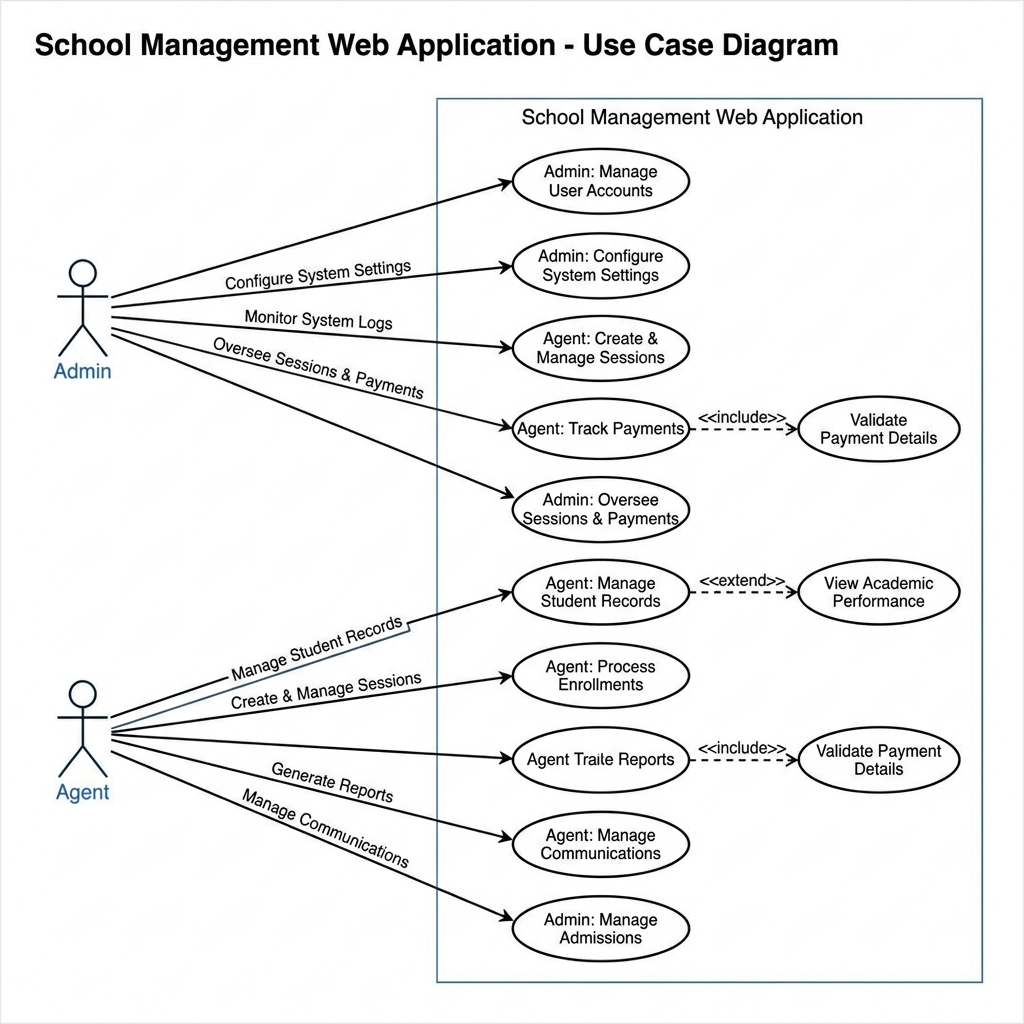
\includegraphics[width=0.85\textwidth]{images/diagramme_usecase.png}
    \caption{Diagramme de cas d'utilisation}
    \label{fig:usecase}
\end{figure}

\subsection{Diagramme de classes}

Le diagramme de classes permet de représenter la structure conceptuelle 
de la plateforme en mettant en évidence les entités principales ainsi 
que leurs relations. Nous avons ainsi réalisé le diagramme présenté à 
la figure~\ref{fig:classes}.

\begin{figure}[H]
    \centering
    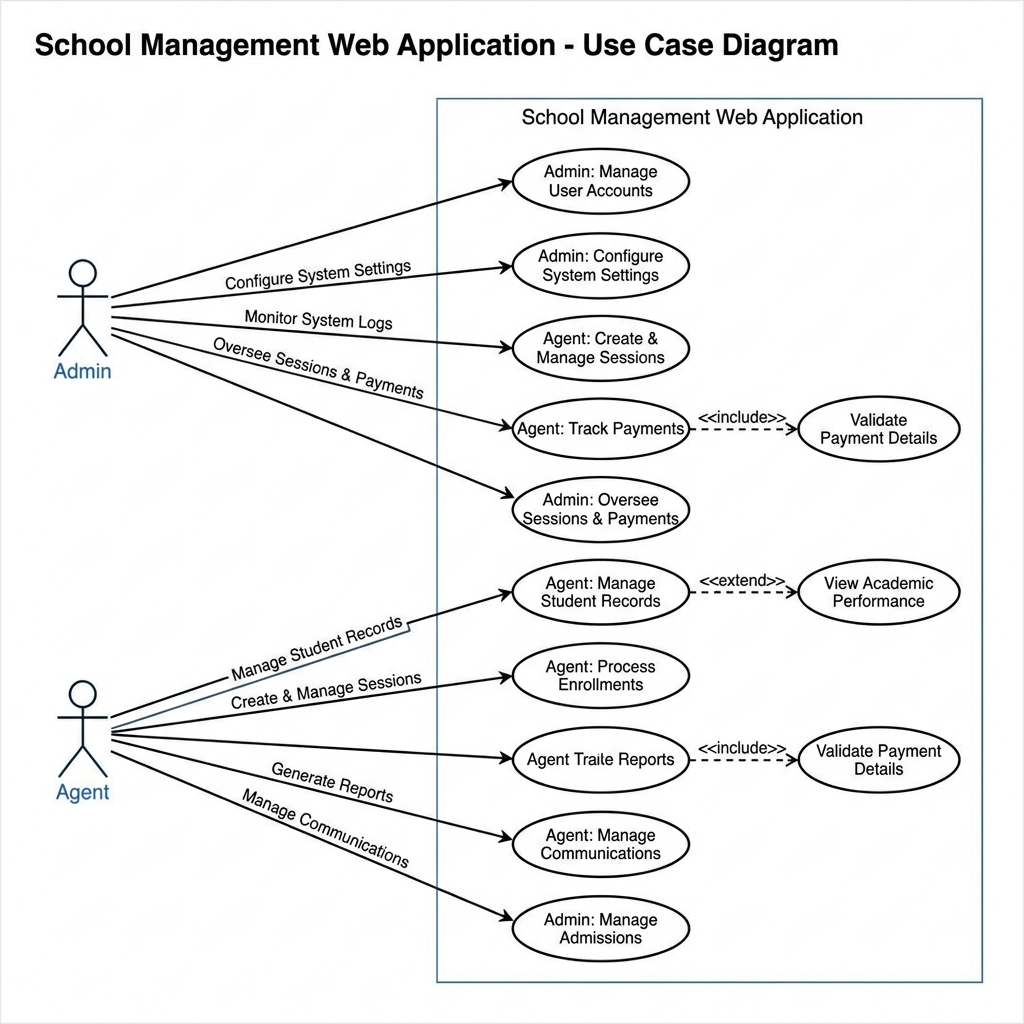
\includegraphics[width=0.85\textwidth]{images/diagramme_classes.png}
    \caption{Diagramme de classes}
    \label{fig:classes}
\end{figure}

\subsection{Diagrammes de séquence}

Le diagramme de séquence illustre de manière dynamique les échanges 
entre les différents objets du système lors de l'exécution de scénarios 
précis. Deux situations essentielles sont modélisées : le processus de 
connexion d'un utilisateur et la création d'une session de travaux 
dirigés.

La figure~\ref{fig:seq1} présente le diagramme de séquence du processus 
de connexion, tandis que la figure~\ref{fig:seq2} illustre le processus 
de création d'une session.

\begin{figure}[H]
    \centering
    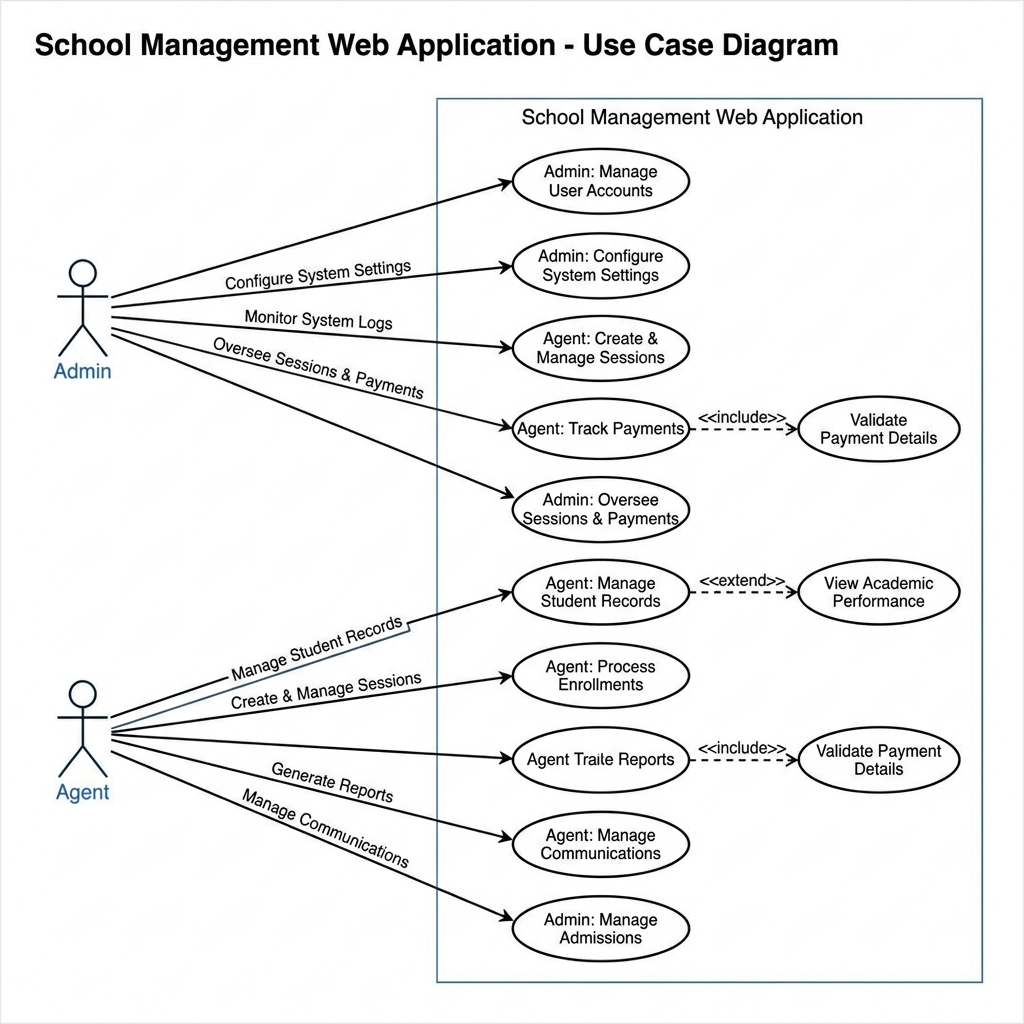
\includegraphics[width=0.85\textwidth]{images/sequence_auth.png}
    \caption{Diagramme de séquence : S'authentifier}
    \label{fig:seq1}
\end{figure}

\begin{figure}[H]
    \centering
    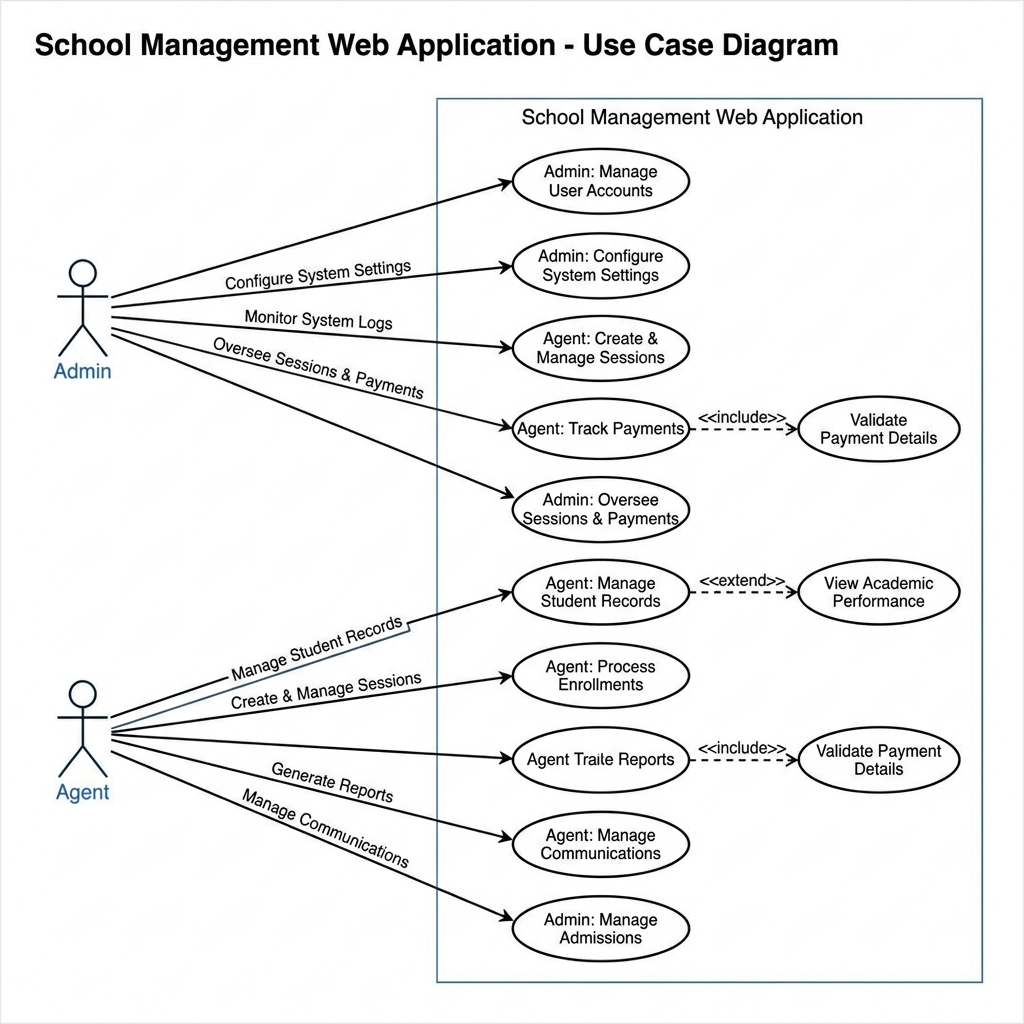
\includegraphics[width=0.85\textwidth]{images/sequence_session.png}
    \caption{Diagramme de séquence : Créer une session}
    \label{fig:seq2}
\end{figure}

% ============================================================
\section{Choix technologiques}
% ============================================================

Ce projet repose sur une architecture moderne fondée sur une séparation 
claire entre le front-end et le back-end. Les choix technologiques ont 
été guidés par des critères de performance, de maintenabilité, de 
sécurité et d'évolutivité.

\subsection{Frontend}

\begin{itemize}
    \item \textbf{HTML5 / CSS3} constituent la base structurelle et 
    visuelle de l'interface. Ils assurent une présentation claire, 
    accessible et compatible avec l'ensemble des navigateurs modernes.

    \item \textbf{JavaScript} assure le dynamisme de l'interface 
    utilisateur, notamment pour les interactions en temps réel, la 
    gestion des formulaires et l'affichage des données du tableau de 
    bord sans rechargement de page.
\end{itemize}

\subsection{Backend}

\begin{itemize}
    \item \textbf{Laravel} est un framework PHP reconnu pour sa 
    robustesse et sa simplicité d'utilisation. Il propose une 
    architecture MVC claire, une gestion avancée de l'authentification 
    et un écosystème riche (migrations, Eloquent ORM, API Resources). 
    Laravel facilite également la sécurisation des données grâce à son 
    système d'authentification moderne et à la gestion des tokens via 
    Sanctum.

    \item \textbf{MySQL} est un système de gestion de base de données 
    relationnelle largement adopté pour sa rapidité, sa fiabilité et sa 
    compatibilité avec de nombreux environnements web. Il permet 
    d'organiser, de stocker et de manipuler efficacement les données, 
    tout en offrant des fonctionnalités de sécurité et de gestion des 
    transactions.
\end{itemize}

% ============================================================
\section*{Conclusion}
\addcontentsline{toc}{section}{Conclusion}
% ============================================================

Ce chapitre a permis de décrire la méthode de conception adoptée pour 
structurer le développement de la plateforme, en s'appuyant sur les 
diagrammes UML pour modéliser les interactions, les entités et les 
scénarios clés. Il a également mis en lumière les choix technologiques 
effectués pour assurer la robustesse, la sécurité et la scalabilité du 
projet. Les résultats de notre travail seront présentés dans le 
chapitre 3.
